\section{Introduction}
%Recent years have witnessed a surge of interest in endowing machines with the ability 
%to acquire knowledge from natural language text. 
%\KZ{Consider changing the title. Very mysterious. You might as well say
%reasoning flow.}
Being capable of comprehending a document and answering a 
question dedicated for the content in the document, often referred as machine reading comprehension(RC) style question answering, is an important and 
challenging task in natural language understanding. The proposal of large-scale single-document datasets, such as CNN/Daily mail~\cite{DBLP:journals/corr/HermannKGEKSB15}, SQuAD~\cite{DBLP:journals/corr/RajpurkarZLL16}, SQuAD2.0~\cite{DBLP:journals/corr/abs-1806-03822}, makes 
training feasible for end-to-end deep neural models~\cite{DBLP:journals/corr/SeoKFH16, DBLP:journals/corr/XiongZS16,Shen2017}. 
The performance on these datasets is further boosted after the release of pre-trained language models such as ELMo~\cite{DBLP:journals/corr/abs-1802-05365} and BERT~\cite{DBLP:journals/corr/abs-1810-04805}. 

\begin{figure}[!htb]
	\centering
	\scalebox{1.0}{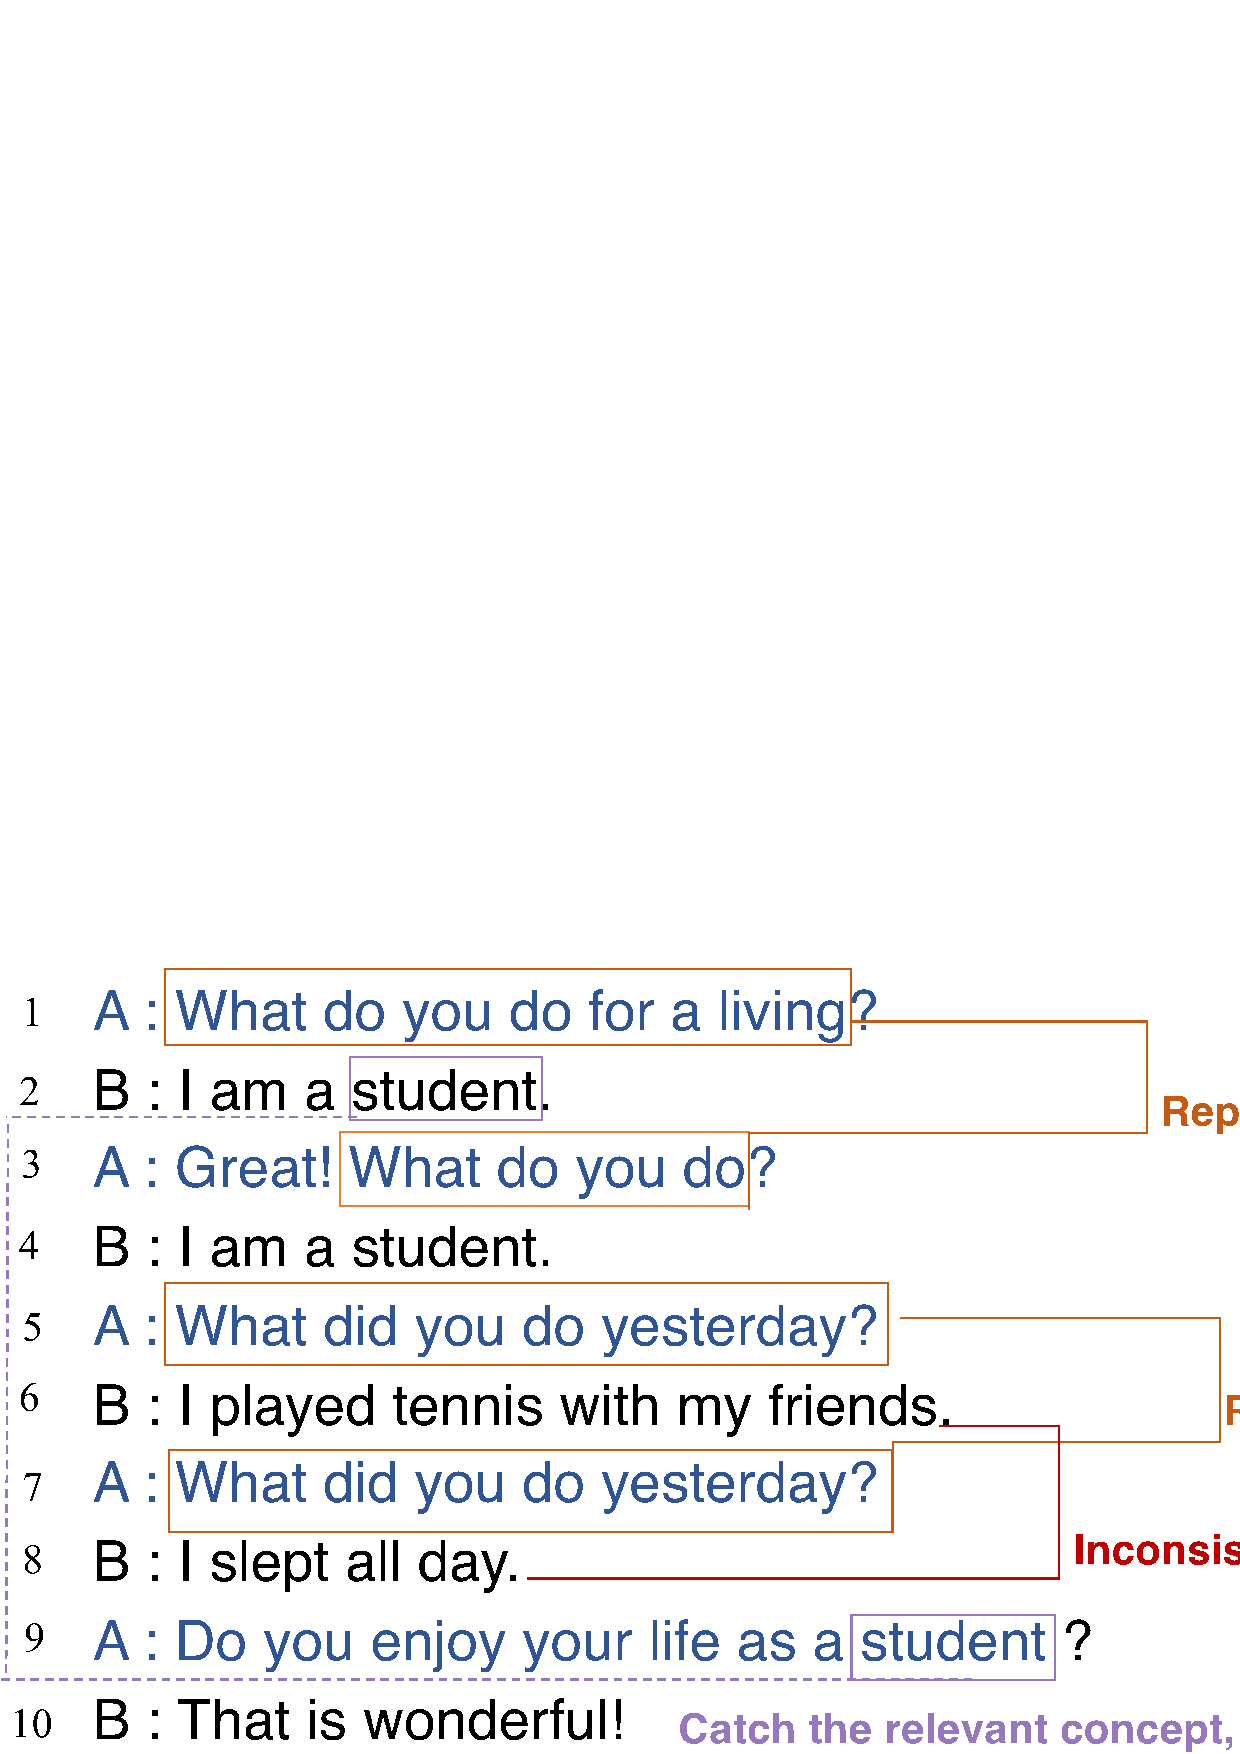
\includegraphics[width=1.0\columnwidth]{figure/example2.jpg}}
	\caption{A multi-hop RC example where an inference path connecting two documents is needed to derive the answer.} \label{fig:example}
\end{figure}
However, it has been observed that most questions in these datasets can be answered relying on information contained in a single sentence~\cite{weissenborn-etal-2017-making}, and gap still
exists between these datasets and real-world situation which requires evidence aggregation and logical reasoning across multiple documents. Therefore, reading comprehension tasks with multiple hops were proposed to realize more sophisticated inference capacity, e.g. WikiHop~\cite{Welbl2018}. Each instance in WikiHop consists of multiple supporting documents, and the goal is to select the correct answer from a set of candidates given a query.
Most queries in the dataset cannot be answered depending on a single document, hence multi-hop reasoning chains across multiple document are needed~(See \figref{fig:example}).
Consequently, previous QA models achieving superior performance on single-document RC datasets are significantly crippled under the multi-hop scenario.

Three lines of approaches have been proposed to tackle this task. The first is extension built upon previous RC models. The earliest attempt \cite{DBLP:journals/corr/abs-1804-05922} is recasting the 
task into a single-document RC problem by concatenating all documents into a sequence and 
establishing skip connections between entities via coreference resolution. 
Co-attention based models~\cite{Zhong2019} explicitly utilize both 
document-level and 
entity-level query-aware representation for candidate selection. 
The second type of research employs graph neural 
networks~(GNN)~\cite{Song2018, Cao2019, Tu2019, BAG} to perform 
multi-step reasoning on various semantic graph via message
passing mechanism. Nodes in the graph are mentions of candidates, 
of which the hidden states are updated by iteratively aggregating 
information from neighboring nodes. 
Reasoning is performed implicitly in these two lines of approach 
and it still remains opaque how answers are derived. 

The third line of work focuses on extracting explicit evidence 
paths using weak supervision~(e.g., location of correct answer) 
to provide more human-interpretable model prediction. \citet{Chen2019} achieves this by constructing document-level reasoning trees. \citet{Kundu2019} considers more fine-grained sequences of named entities as evidence by extracting subsequent entities in proximal cotext step-by-step. However, none of them 
are able to perform human-like reasoning behavior with grounded 
semantics such as \textit{who did what to whom}.
%\KZ{Give a little example how they
%did it and why their way of interpretation is insufficient?}
%Nevertheless, most of existing models still remain black boxes with little to none interpretation of model prediction. 

To overcome the limitations of previous methods, in this paper we propose Reasoning Flow (RF), a novel graph-based method which also falls under the third category. 
%while being able to recover evidential reasoning path with fine-grained semantic compositionality. 
RF accomplishes interpretable multi-hop reading comprehension by abstracting textual 
information present in documents and query into relational graph with fine-grained semantics and identifying evidential paths on the graph that lead to the predicted answer.
RF is different from previous interpretable methods mainly in that it is able to 
discover reasoning paths with fine-grained relation 
automatically through end-to-end training.
Specifically, equipped with a newly-designed two-stream collaborative node representation 
learning mechanism, RF has the following advantages:
\begin{itemize}
    \item Compared to previous graph-based models which mainly consider mentions of candidates as nodes, 
the RF graph jointly model mentions of candidates, coreferent pronouns and relevant bridge entities 
with six types of edges to capture multi-granularity levels of semantic relation 
within and cross concepts.
    \item The proposed collaborative graph representation learning mechanism involves alternate 
execution of a relational message passing step and a coarse-to-fine reasoning path 
induction step at each hop, the output of which is able to recover potentially 
more-than-one inference chains with fine-grained semantic compositionality 
via backward beam search decoding.
    \item The reasoning path induction module is learned end-to-end 
based on the constructed semantic graph through computationally efficient matrix operation, 
exempting the need of brute-force enumeration over all possible paths as in ~\cite{Kundu2019}.
\end{itemize}  

Through comprehensive experiments, we show that our proposed model can 
achieve comparable or better performance than previously published multi-hop RC models 
while being able to produce explanations in the form of explicit paths 
with fine-grained semantics that are shown to be reasonable by human evaluation. 
%\KZ{Make the contributions more concrete by adding some numbers or adjectives.}
